\documentclass[twoside,12pt]{wipb}
\usetikzlibrary{mindmap,trees}%dla diagramu Computer science mindmap

\usepackage{url}
\usepackage{float}
\usepackage{paralist}
\usepackage{xcolor}
\usepackage[nottoc,numbib]{tocbibind}

\widowpenalty=10000
\clubpenalty=10000

\raggedbottom

\katedra{OPROGRAMOWANIA}
\typpracy{ inżynierska
           %inżynierska
         }

\temat{APLIKACJA MOBILNA DO ZARZĄDZANIA TRENINGIEM NA SIŁOWNI}
\autor{Norbert Kamieński}
\promotor{dr inż. Marcin Czajkowski}
\indeks{93401}

\studia{stacjonarne
        %niestacjonarne
       }

\rokakademicki{2016/2017}

\profil{%magisterskie jednolite
        %magisterskie uzupełniające
        %studia I stopnia
        studia I stopnia
}
\kierunekstudiow{informatyka
                 %matematyka
                }

\specjalnosc{ 
             %Inżynieria Komputerowa
             %Systemy Oprogramowania
             %Metody infnformatyczne w~banknkowości i~finansach
             %Ochrona systemów informatycznych
            }

\zakres{1. Opis technologii wykorzystywanych przy tworzeniu systemu.  \newline
 2. Wykonanie projektu aplikacji do zarządzania treningiem na siłowni.   \newline 
 3. Implementacja i testy zrealizowanej aplikacji.  \newline }
\slowakluczowe{Aplikacja Mobilna, React Native, Firebase, JavaScript, Android, Organizer }


\hypersetup{ %wpisy w pdf info
pdfauthor={Norbert Kamieński},
pdftitle={Aplikacja mobilna do zarządzania treningiem na siłowni},
pdfsubject={Organizer usprawniający osobom trenującym prowadzenie oraz monitorowanie własnych treningów.},
pdfkeywords={Aplikacja Mobilna, React Native, Firebase, JavaScript, Android, Organizer},
pdfpagemode=UseNone,
linkcolor=black,
citecolor=black
} 

\begin{document}
\maketitle
\chapter*{Mobile application to manage training in the gym}

Major goal of this thesis was to create a mobile application that helps athletes manage their trainings in the gym. For this purpose has been designed and developed mobile application. It is easier way to organize and track the progress of sportsmen workouts.
Humans memory is an unreliable. Athletes have a problem with that as well. Trainees don’t remember what weight recently trained or how series, reps they lifted. Somebody note that in a usual notebook. But It is not very handy, can be forgot it and have limited space.
That application solves these and many others problems. Most people have a mobile at this moment, which takes to the gym, too. Software allows to note progress during training and planning or observing some statistic.
Application is programmed in the JavaScript’s framework React Native supported by Redux technology. Framework uses functional approach to programming and frontends technologies like HTML, JSX and CSS. Although used web technologies, application is 100% native.
The paper contains five chapters. The first is an introduction. It presents the goal, plan and scope of work. Second chapter- shows an overview of the application, existing solutions and functional and nonfunctional requirements. The most important fourth chapter describes implementations project. It contains application architecture, principle of operation, tests and product presentations. The last is summary of the work.
Finally created the application, already used by athletes.


\tableofcontents
\thispagestyle{empty}
\setcounter{page}{0}
\pagestyle{plain}

\addtocontents{toc}{\protect\thispagestyle{empty}}

\chapter[Wstęp.]{Wstęp}

\section{Cel pracy}

\section{Zakres pracy}

\section{Plan pracy}

\chapter[Analiza wymagań.]{Analiza wymagń}

\section{Wizja oraz ogólny zarys aplikacji.}
Głównym celem powstania aplikacji jest pomoc osobom trenującym w organizacji ich treningu na siłowni. 

Często spotykanym zjawiskiem jest zapominanie ostatnio wykonywanych treningów. Zwłaszcza początkujący ale i również doświadczone osoby mają problemy z zapamiętaniem trenowanych ćwiczeń, przenoszonego obciążenia czy też zakresu powtórzeń.

Trenujący próbują rozwiązać ten problem poprzez notowanie progresu w zeszycie.
Nie rozwiązuje to jednak do końca problemu. Nierzadko przytrafia się zapomnienie notesu, długopisu a same targanie wraz z innymi akcesoriami treningowymi nie należy do przyjemnych. Posiada on również ograniczone miejsce oraz jest podatny na uszkodzenia.

Najodpowiedniejszym rozwiązaniem problemów wydaje się być aplikacja mobilna. Jedyną rzeczą jaką użytkownik musi zrobić, to wziąć swój telefon na trening. Służy nam on w różnych aspektach życia co sprawia, że trudno go zapomnieć.

Aplikacja będzie nieskomplikowana oraz niezbyt przeładowana. Posiadać będzie czytelny interfejs. Najważniejszą przewidzianą funkcją ma być archiwizacja danych oraz notowanie aktualnego treningu. Ważnym dodatkiem będzie lista ćwczeń zawierająca opis każdego z nich. Zakładka ulubione ćwiczenia- pomoże łatwiej je pogrupować oraz odszukać użytkownikowi. Usprawnieniem treningu będzie minutnik, który pomoże precyzyjnie odmieżać czas wykonywanego interwału lub przerwy między seriami lub ćwiczeniami. Ponadto każdy z użytkowników będzie posiadał własne staystyki, możliwe do obserwacji na rysowanych wykresach. Ćwiczący będzie miał możliwość obliczania swojego maksymalnego powtórzenie oraz progresji falowej. W kwesti statystyk program będzie udostępniał również narzędzie do monitorowania zmiany wagi, uzależnione od objętości treningu oraz spożywanych kalorii.

\section{Istniejące rozwiązania.}

Jeszcze nie dawno w sieci trudno było dostrzec apliakcje mobilne wspomagających trening. W danej chwili rynek obfituje w podobne do projektowanego rozwiązania. Moda społeczeństwa na bycie wysportowanym, sprawnym fizycznie sprawiła powstanie wielu podobnych programów. W niedalekiej przeszłości dostępne były tylko i wyłącznie aplikacje internetowe, które użytkownik musiał uzupełniać dopiero po skończonym treningu.

Do sieci trafiło wiele aplikacji, mniej lub bardziej skomplikowanych. Jedna z nich to StrongLifts. Jest to bardzo przyjemna dla użytkownika aplikacja, posiadająca przyjazny interfejs graficzny. Nie jest również przaładowana zbyt dużą ilością funkcjonalności. Posiada jednak swoje ograniczenia. Trening możemy przeprowadzać wyłącznie w schemacie  '5x5' oraz zawiera małą listę ćwiczeń.

Podobną aplikacją jest również GymRun. Bardzo prosta w obsłudze, udostępniając do tego wiele możliwości. Umożliwia tworzenie własnych planów treningowych, śledzenie progresji oraz dokumentację składu ciała. Brakuje jej jednak opcji kalkulowania miesięcznej progresji, obliczonej od maksymalnego powtórzenia.  Inną wadą są braki opisania ćwiczenia. Uniemożliwia to początkującemu naukę poprawnej techniki wykonania. Nowy użytkownik nie potrafi ocenić swoich zdolności, co często prowadzi do kontuzji lub przetrenowania.

FitNotes to kolejna aplikacja w tym zestawieniu. Interfejs graficzny nie przyciąga oka, dodatkowo sprawia wrażenie nieintuicyjnego. Aplikacja udostępnia ogromną ilość funkcji oraz opcji, co jednak przy mobilnych gabaytach urządzenia nie wpływa na wygodę korzystania. Wykorzystanie w organizerze tylko języka angielskiego, przy braku opisania ćwiczeń może sprawiać niektórym problem.

Poniżej zamieszczone są przykładowe zrzuty ekranu przedstawionych aplikacji.

\begin{figure}[H]
\centering
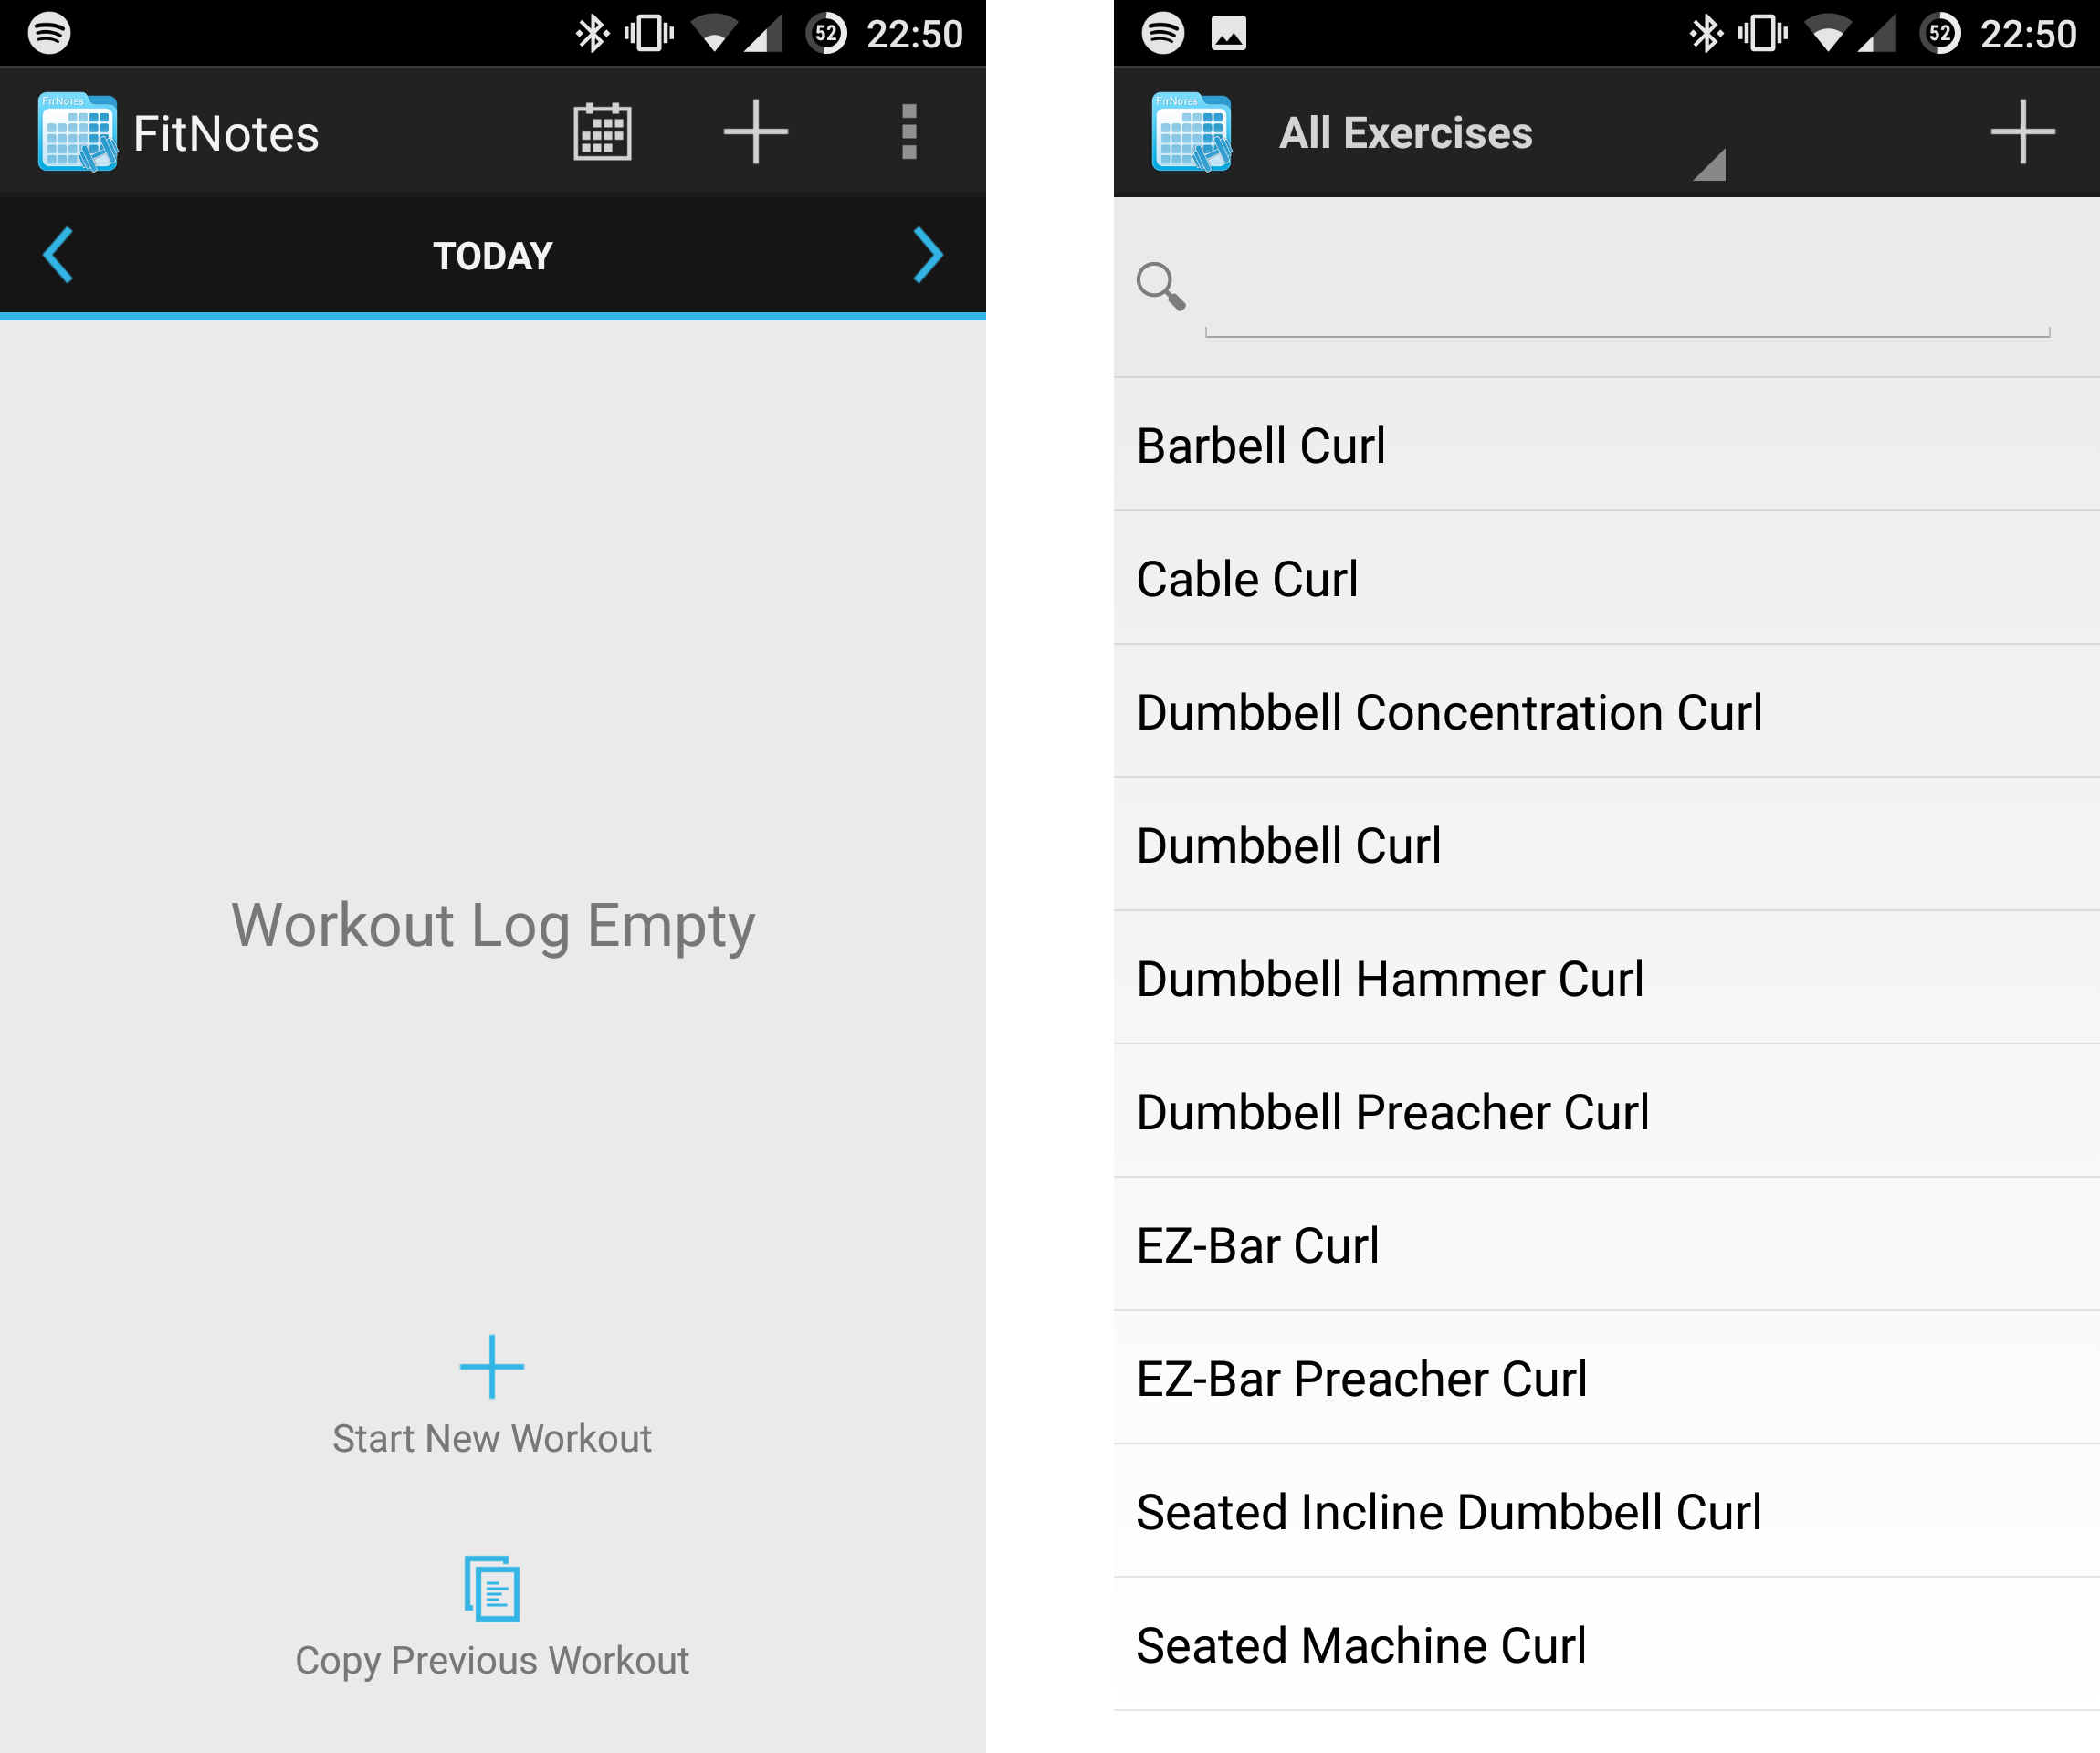
\includegraphics[width=\textwidth, keepaspectratio=true]{grafika/istn1.jpg} 
	\caption{ FitNotes }
\end{figure}

\begin{figure}[H]
\centering
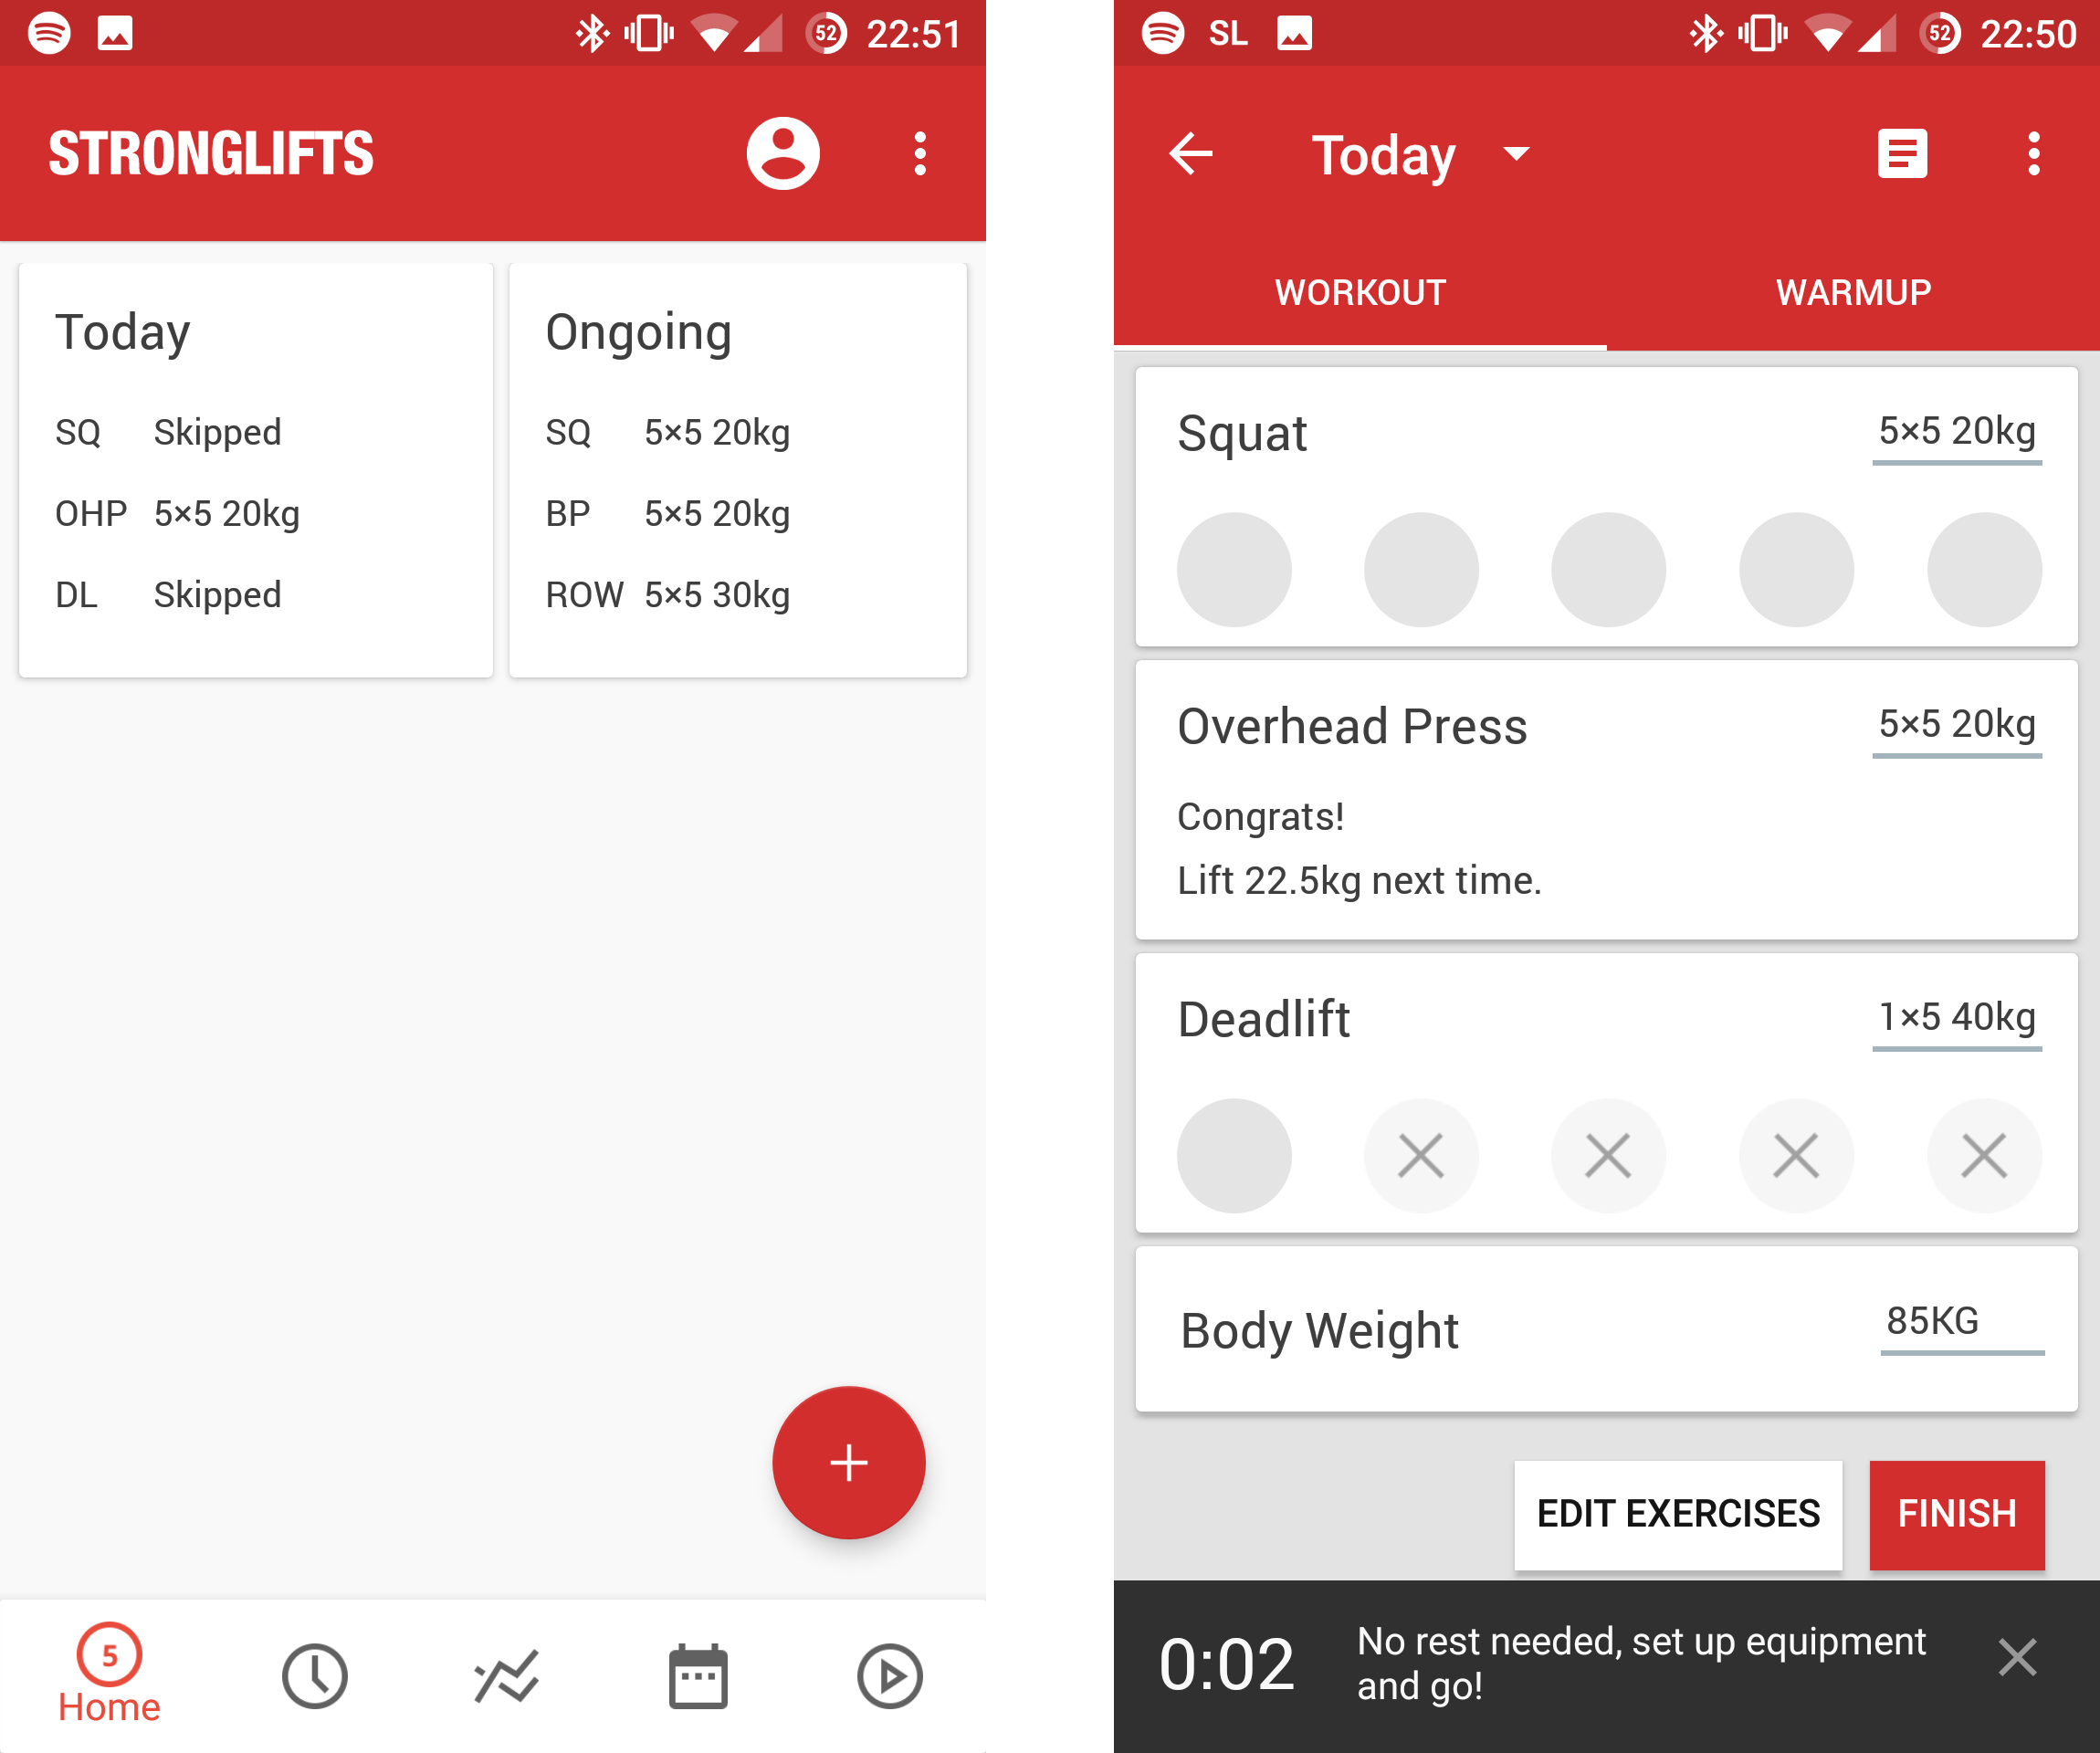
\includegraphics[width=\textwidth, keepaspectratio=true]{grafika/istn2.jpg} 
	\caption{ StrongLifts }
\end{figure}

\begin{figure}[H]
\centering
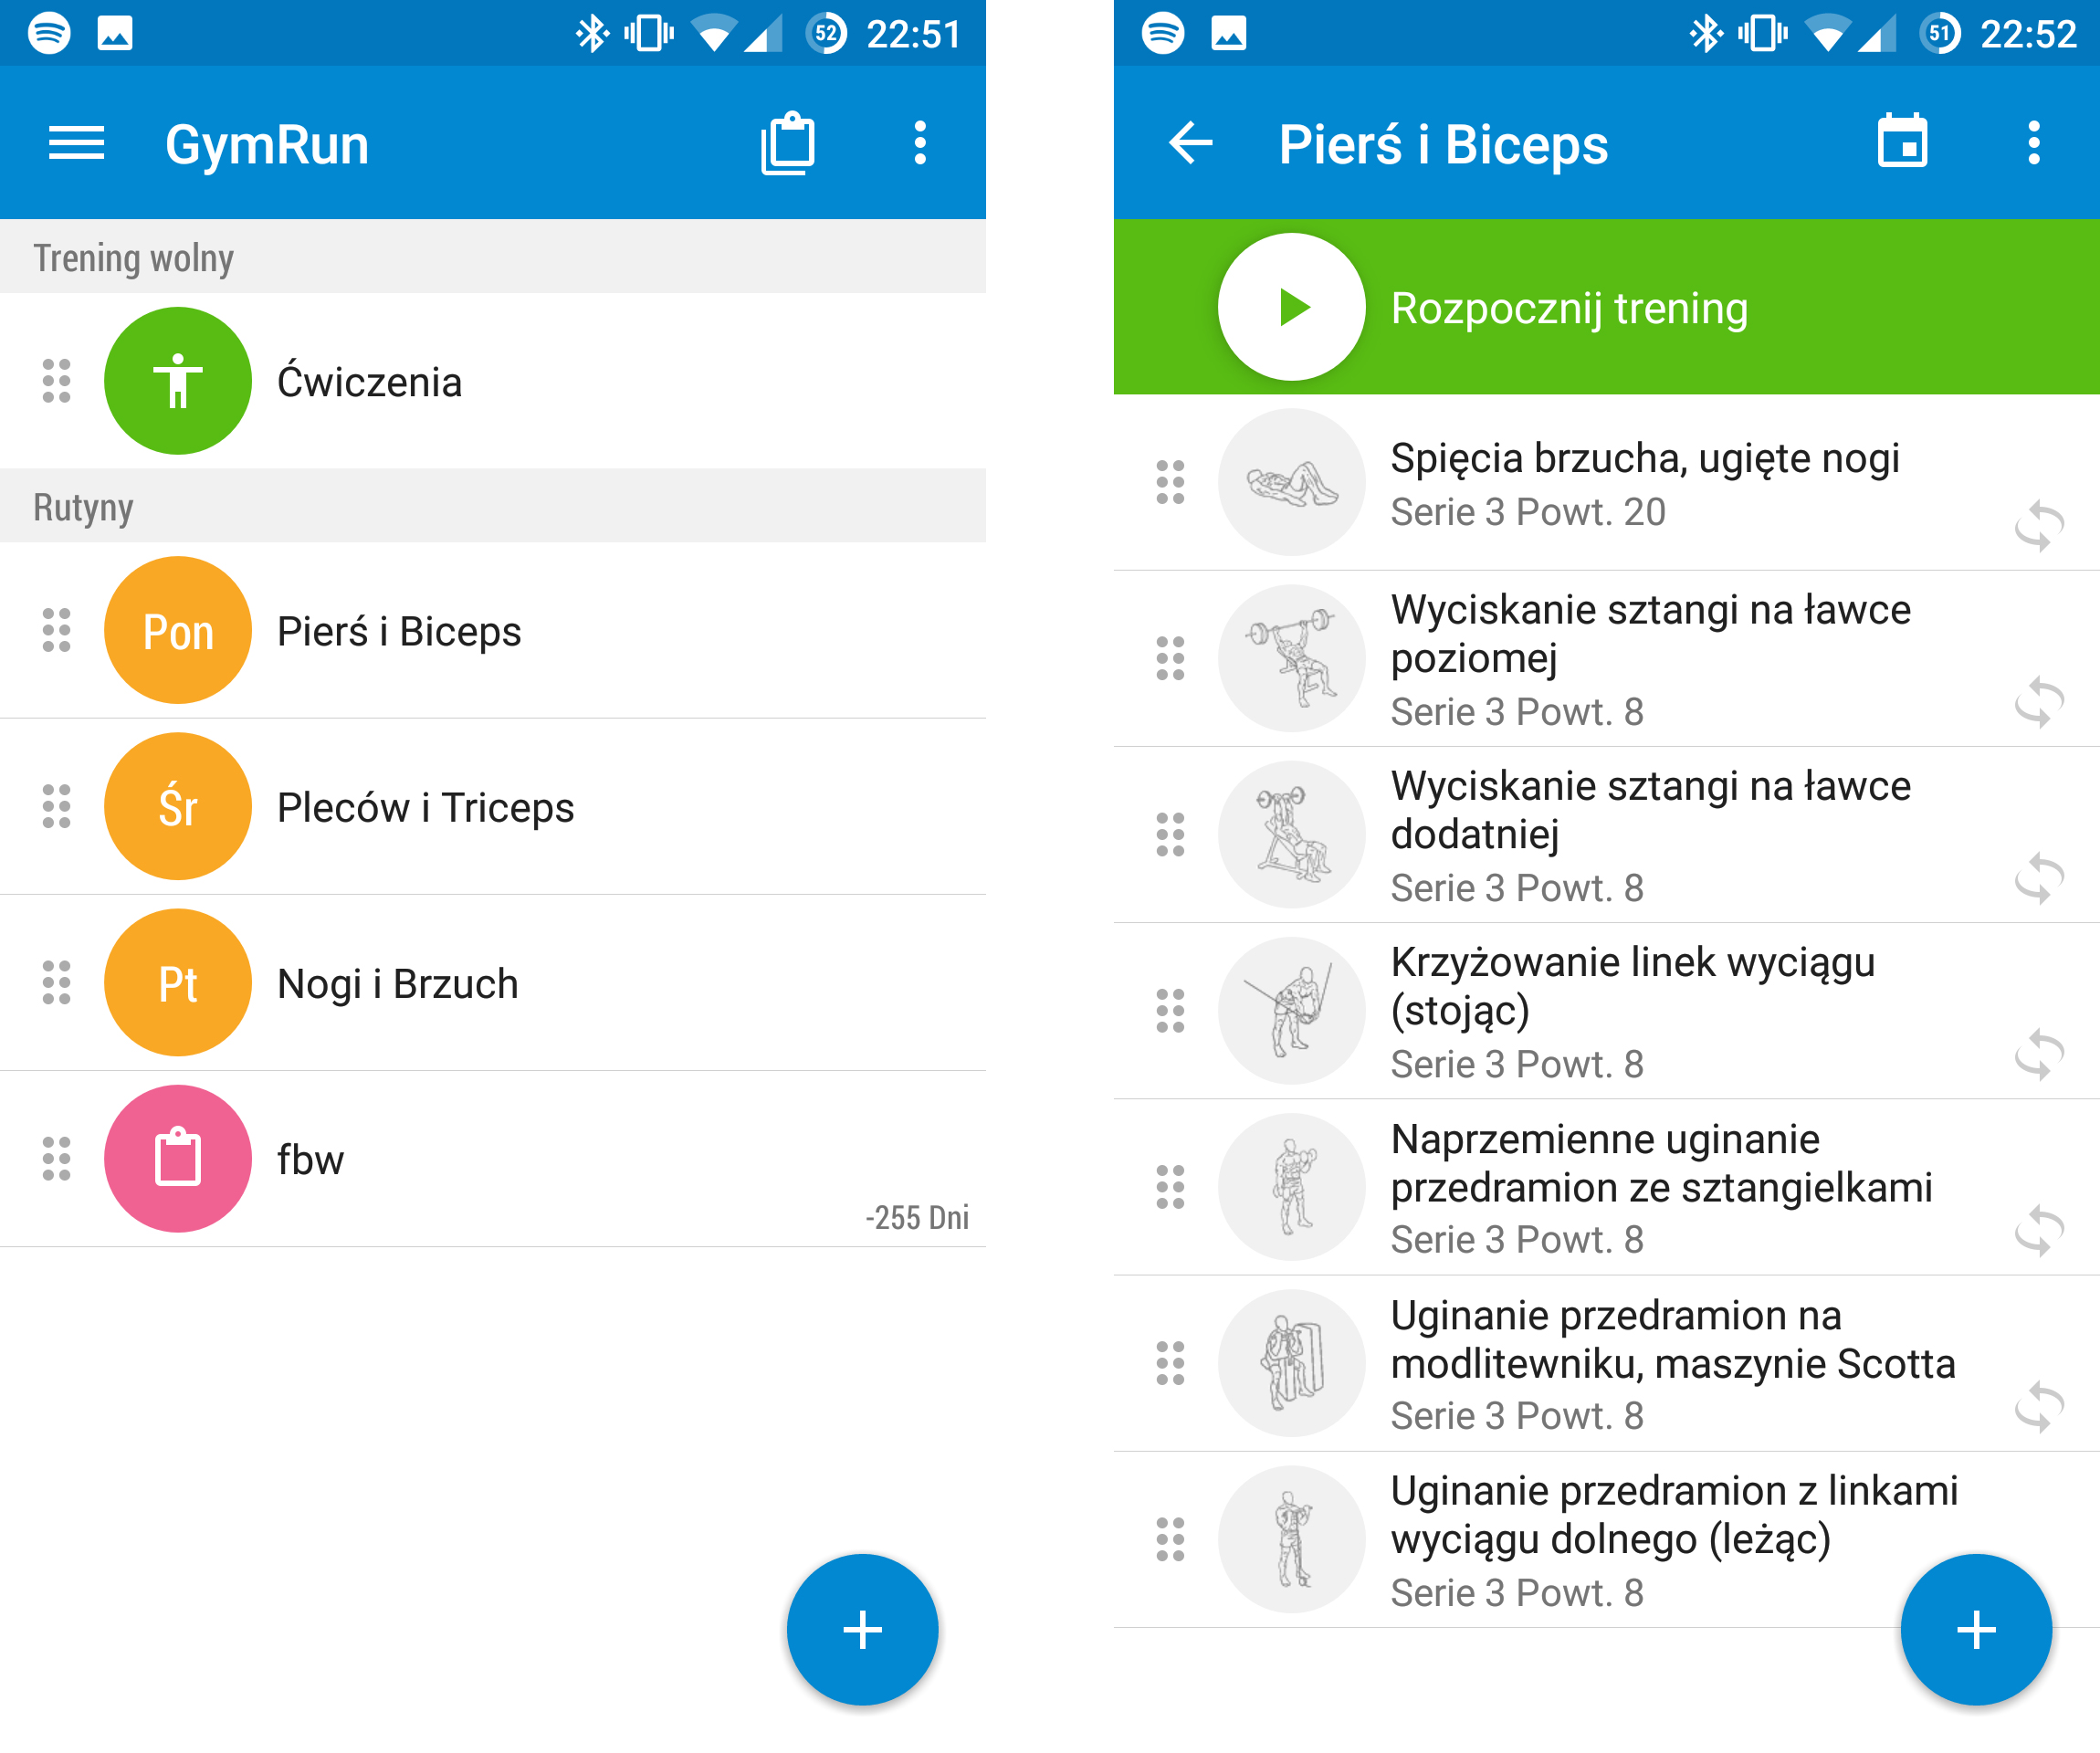
\includegraphics[width=\textwidth, keepaspectratio=true]{grafika/istn4.jpg} 
	\caption{ GymHero }
\end{figure}
\newpage

Opis najważniejszych z nich.

Opis przypadku użycia "Przypadek użycia"

\begin {enumerate}
\item Uczestniczący aktorzy.
\begin {enumerate}
\item Użytkownik
\end {enumerate}
\item Podstawowy ciąg zdarzeń
\begin {enumerate}
\item raz
\item dwa
\item trzy
\item cztery
\end {enumerate}
\item Alternatywne ciągi zdarzeń
\begin {enumerate}
\item raz
\begin {itemize}
\item aaaa
\end {itemize}
\item dwa
\begin {itemize}
\item bbbb
\end {itemize}
\end {enumerate}
\item Zależności czasowe
\begin {enumerate}
\item raz:
\item dwa:
\item trzy:
\item cztery:
\end {enumerate}
\item Wartości uzyskane przez aktorów po zakończeniu przypadku użycia
\begin {enumerate}
\item raz:
\end {enumerate}
\end {enumerate}

\section{Wymagania funkcjonalne}

Analiza wymagań jest najważniejszym elementem kreowania aplikacji. W każdym procesie tworzenia projektu powina być przeprowadzana w pierwszej kolejności. Zebrane są tu wszystkie funkcjonaloności udostępniane przez aplikacje mobilną. Wymagania funkcjonalne potrafią ukazać usługi oraz cechy oferowane przez produkt. Szczegółowy opis został przedstawiony za pomocą diagramu przypadków użycia aplikacji oraz opisów kilku z nich. Całość kończy lista wymagań, którą powinna potrafić wykonać aplikacja.

\begin{figure}[H]
\centering
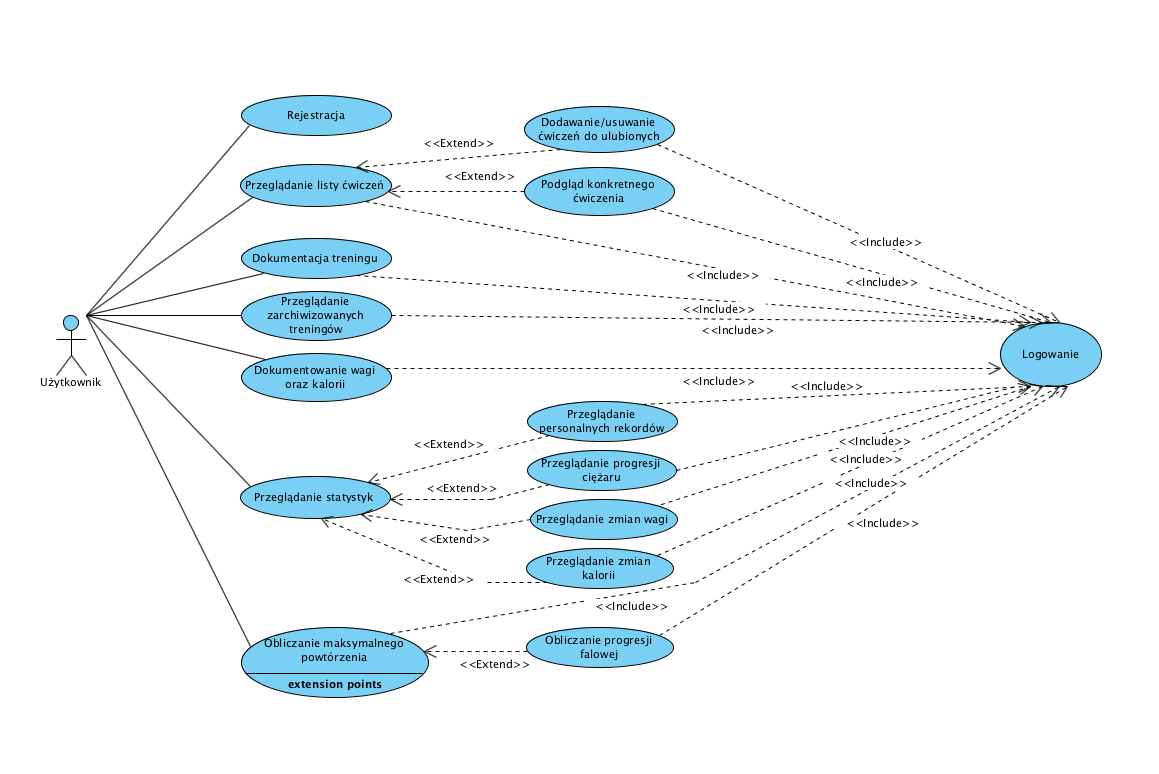
\includegraphics[width=\textwidth, keepaspectratio=true]{grafika/diagram_przebiegu.png} 
	\caption{ Diagram czynności }
\end{figure}
\newpage

\section{Wymagania niefunkcjonalne}
\chapter[Wykorzystane technologie.]{Wykorzystane technologie}

\section{Przegląd technologii}

\subsection{Swift (Objectiv-C)}
 
\subsection{Android (Java)}
 
\subsection{React Native (Javascript)} 

\section{Wybrane technologie}

\subsection{React Native + Redux}

\subsection{Javascript (JSX, ES6)}

\subsection{HTML  \& CSS}

\subsection{Firebase.}

\section{Wybrane technologie.}

\subsection{Microsoft Visual Studio.}

\subsection{React Native Debugger.}

\subsection{GIT- system kontorli wersji.}
\chapter[Realizacja aplikacji.]{Realizacja aplikacji}

\section{Architektura aplikacji mobilnej}

\section{Schemat działania aplikacji}

\section{Baza danych}

\section{Prezentacja aplikacji}

\section{Testy aplikacji}

\section{Wdrożenie}

\section{Obsługiwane systemy monitorowania}
\chapter[Podsumowanie]{Podsumowanie}

%\chapter[Bibliografia.]{Bibliografia}

%\chapter[Podsumowanie]{Podsumowanie}


\nocite{*} %wszystkie wpisy w bibliografi
\bibliographystyle{unsrt} %{latex8} posortowane wzgledem wystepowania
\bibliography{bibliografia}%

%\addtocontents{toc}{\contentsline {chapter}{Bibliografia}{\thepage}{}}
\listoftables
%\addtocontents{toc}{\contentsline {chapter}{Spis tabel}{\thepage}{}}
\listoffigures
%\addtocontents{toc}{\contentsline {chapter}{Spis rysunków}{\thepage}{}}
\lstlistoflistings
%\addtocontents{toc}{\contentsline {chapter}{Spis listingów}{\thepage}{}}
%\listofalgorithms % w zaleznosci od kompilatora i wersji klasy moga wystapic bledy przy kompilacji
%\addtocontents{toc}{\contentsline {chapter}{Spis algorytmów}{\thepage}{}}

\newpage
\thispagestyle{empty}
\mbox{}
\biblioteka{tak} % tak/nie
\end{document}
